\section{2-qubits PCE quantum channels}\label{sec:2_qubits}
Próximamente...

\begin{figure}
\centering
\includegraphics[width=\linewidth]{two_qubits_generators_diagrams}
\begin{tikzpicture}[x=1mm,y=1mm,overlay,remember picture]
%    \pgftransformshift{\pgfpointanchor{current page}{center}}
\node[inner sep=0pt] (usac) at (-38.5,17) {$\mcG_{(0,0)}$};
\node[inner sep=0pt] (usac) at (-27.5,17) {$\mcG_{(0,1)}$};
\node[inner sep=0pt] (usac) at (-16.5,17) {$\mcG_{(0,2)}$};
\node[inner sep=0pt] (usac) at (-5.5,17) {$\mcG_{(0,3)}$};
\node[inner sep=0pt] (usac) at (5.5,17) {$\mcG_{(1,0)}$};
\node[inner sep=0pt] (usac) at (16.5,17) {$\mcG_{(1,1)}$};
\node[inner sep=0pt] (usac) at (27.5,17) {$\mcG_{(1,2)}$};
\node[inner sep=0pt] (usac) at (38.5,17) {$\mcG_{(1,3)}$};
\node[inner sep=0pt] (usac) at (-38.5,1) {$\mcG_{(2,0)}$};
\node[inner sep=0pt] (usac) at (-27.5,1) {$\mcG_{(2,1)}$};
\node[inner sep=0pt] (usac) at (-16.5,1) {$\mcG_{(2,2)}$};
\node[inner sep=0pt] (usac) at (-5.5,1) {$\mcG_{(2,3)}$};
\node[inner sep=0pt] (usac) at (5.5,1) {$\mcG_{(3,0)}$};
\node[inner sep=0pt] (usac) at (16.5,1) {$\mcG_{(3,1)}$};
\node[inner sep=0pt] (usac) at (27.5,1) {$\mcG_{(3,2)}$};
\node[inner sep=0pt] (usac) at (38.5,1) {$\mcG_{(3,3)}$};
\end{tikzpicture}
\caption{PCE generators of 2 qubits.}
\end{figure}


